\documentclass[10pt,a4paper]{article}
\usepackage[a4paper,top=16mm,bottom=16mm,left=18mm,right=18mm,footskip=8mm]{geometry}
\usepackage{fontspec}
\setmainfont{Liberation Sans}[BoldFont={Liberation Sans Bold},ItalicFont={Liberation Sans Italic}]
\usepackage{xcolor,tikz,tcolorbox,tabularx,booktabs,enumitem,fancyhdr,graphicx}
\usetikzlibrary{arrows.meta,calc}
\tcbuselibrary{skins,breakable}
\usepackage[ngerman,provide=*]{babel}
\usepackage{hyperref}
\hypersetup{hidelinks,pdftitle={Wo trage ich At price ein? – Kurz-Guide},pdfauthor={}}

\definecolor{buy}{HTML}{17784A}   \definecolor{sell}{HTML}{A52A1F}
\definecolor{ink}{HTML}{16181D}   \definecolor{muted}{HTML}{6B7280}
\definecolor{soft}{HTML}{9CA3AF}  \definecolor{rule}{HTML}{E5E7EB}
\definecolor{greya}{HTML}{9AA1AB} \definecolor{tintblue}{HTML}{F3F6FB}
\definecolor{tintpeach}{HTML}{FBF5F2} \definecolor{boxbg}{HTML}{F7F8FA}
\definecolor{text2}{HTML}{33383F}
\definecolor{wbg}{HTML}{0E2939} \definecolor{whead}{HTML}{0B2130} \definecolor{wfield}{HTML}{102B3C}
\definecolor{wborder}{HTML}{1D4256} \definecolor{waccent}{HTML}{1B6CA8} \definecolor{wgreen}{HTML}{3CB44A}
\definecolor{wtext}{HTML}{E7EEF2} \definecolor{wmuted}{HTML}{8FA6B3} \definecolor{wmark}{HTML}{3F88BD}
\definecolor{wdim}{HTML}{5F7A89} \definecolor{wtog}{HTML}{33505F} \definecolor{wknob}{HTML}{C3D2DA}
\definecolor{wred}{HTML}{E0524D} \definecolor{wchart}{HTML}{0B2030} \definecolor{wpill}{HTML}{5B6B76}
\definecolor{wtabtext}{HTML}{CDDBE3} \definecolor{wbadge}{HTML}{0B3A17}

% ---- Schriftgrößen laut Vorgabe ----
\newcommand{\hone}{\fontsize{13.5}{16.5}\selectfont\bfseries}
\newcommand{\htwo}{\fontsize{10.5}{13}\selectfont\bfseries}
\newcommand{\fine}{\fontsize{7.4}{9.2}\selectfont}
\newcommand{\foot}{\fontsize{6.2}{7.6}\selectfont}
\newcommand{\wfont}{\fontsize{6.8}{8}\selectfont}
\newcommand{\wsmall}{\fontsize{5.8}{7}\selectfont}
\newcommand{\ls}{\addfontfeatures{LetterSpace=16}}
\renewcommand{\baselinestretch}{1.22}
\color{ink}\setlength{\parindent}{0pt}\setlength{\parskip}{0pt}

\newcommand{\eyebrow}[1]{{\fine\bfseries\ls\color{muted}\MakeUppercase{#1}}\par\vspace{1.5mm}}
\newcommand{\Hone}[1]{{\hone #1}\par\vspace{2.5mm}}
\newcommand{\Htwo}[1]{{\htwo\ls\color{muted}\MakeUppercase{#1}}\par\vspace{3mm}}
\newcommand{\lead}[1]{{\color{text2}#1}\par}
\newcommand{\hr}{\par\vspace{4.5mm}{\color{rule}\rule{\linewidth}{0.4pt}}\par\vspace{3.5mm}}
\newcommand{\hd}[1]{{\foot\bfseries\ls\color{soft}\MakeUppercase{#1}}}

\newtcolorbox{card}{enhanced,colback=white,colframe=rule,boxrule=0.4pt,arc=2mm,
  left=4mm,right=4mm,top=3.5mm,bottom=3.5mm,boxsep=0pt,before skip=4mm,after skip=0pt}
\newtcolorbox{merk}{enhanced,colback=boxbg,colframe=boxbg,boxrule=0pt,arc=0pt,
  borderline west={2.2pt}{0pt}{ink},left=5mm,right=4mm,top=3mm,bottom=3mm,boxsep=0pt,before skip=4mm,after skip=0pt}
\newtcolorbox{note}[2]{enhanced,colback=boxbg,colframe=boxbg,boxrule=0pt,arc=1.2mm,left=3mm,right=3mm,top=2.5mm,bottom=2.5mm,
  boxsep=0pt,before skip=3mm,after skip=3mm,before upper={{\foot\bfseries\ls\color{#1}#2}\par\vspace{1mm}}}
\newtcolorbox{prule}[1]{enhanced,colback=white,colframe=rule,boxrule=0.4pt,arc=1.2mm,borderline west={2.2pt}{0pt}{#1},
  left=4mm,right=3mm,top=2.3mm,bottom=2.3mm,boxsep=0pt,before skip=2mm,after skip=0pt}
\newtcolorbox{plain}{enhanced,colback=white,colframe=rule,boxrule=0.4pt,arc=2mm,left=4mm,right=4mm,top=3mm,bottom=3mm,boxsep=0pt}
\newlist{steps}{enumerate}{1}
\setlist[steps]{label=\textcolor{\stepcol}{\bfseries\arabic*},leftmargin=6mm,labelsep=2.5mm,itemsep=1.6mm,parsep=0pt,topsep=0pt,font=\color{text2}}
\newcommand{\stepcol}{ink}
\newenvironment{stepsx}[1]{\renewcommand{\stepcol}{#1}\begin{steps}}{\end{steps}}

\pagestyle{fancy}\fancyhf{}\renewcommand{\headrulewidth}{0pt}
\fancyfoot[C]{\foot\color{soft}\thepage}
\newcommand{\cnum}[1]{\tikz[baseline=-0.7ex]\node[circle,fill=ink,text=white,inner sep=0,minimum size=4.2mm,font=\bfseries\fontsize{6.5}{7}\selectfont]{#1};}
\begin{document}

\thispagestyle{empty}
\eyebrow{Trading-Grundlagen · visuell erklärt}
\Hone{Wo trage ich „At price“ ein?}
{\color{ink}\rule{52mm}{1.6pt}}\par\vspace{4mm}
\begin{minipage}{118mm}\lead{Die vier Typen unter „New Pending Order“ auf einen Blick: wo dein At-price-Wert liegt,
wohin der Kurs laufen muss, damit die Order auslöst – und wohin er danach laufen soll.}\end{minipage}
\vspace{18mm}
\begin{plain}{\foot\bfseries\ls\color{soft}ALLE VIER TYPEN AUF EINER PREIS-LEITER}\par\vspace{5mm}
\hspace{8mm}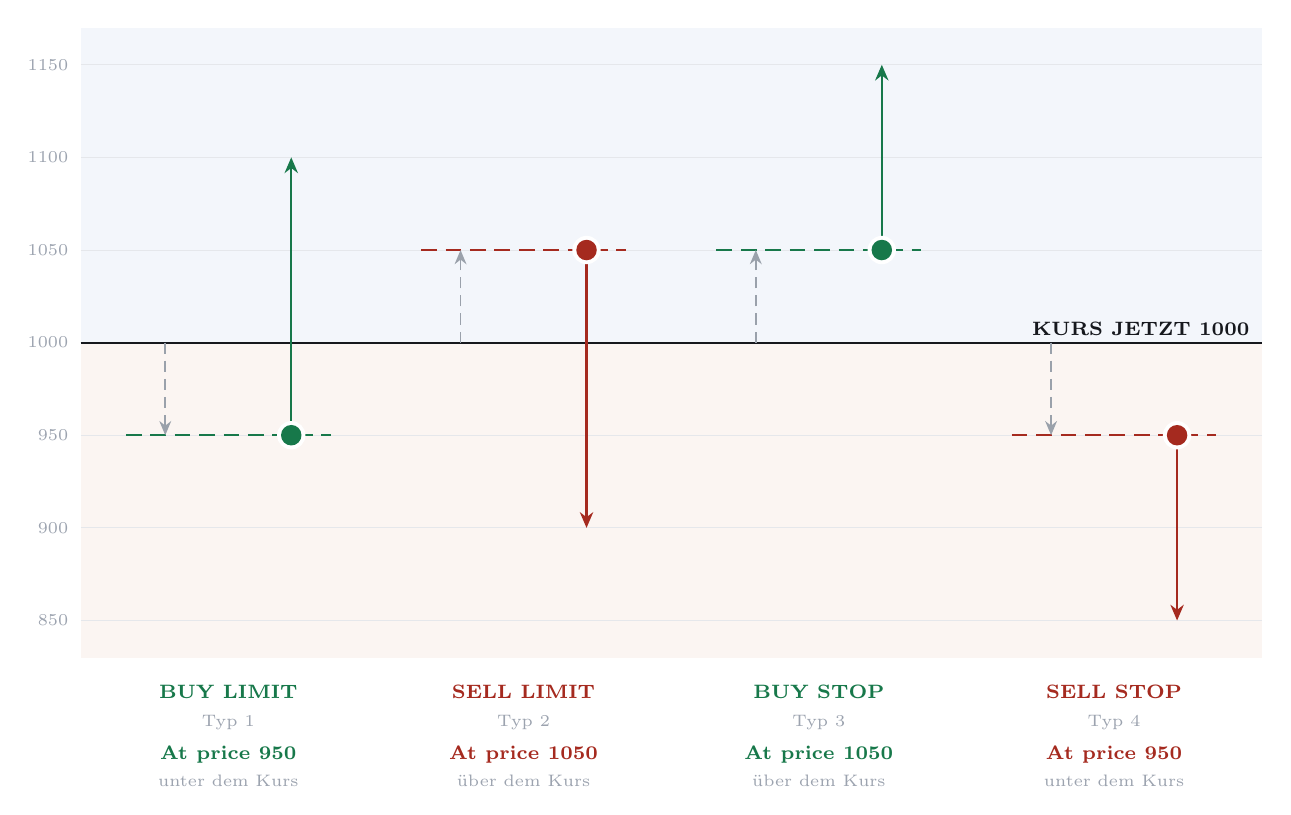
\begin{tikzpicture}[x=1mm,y=1mm,font=\fine]
\fill[tintblue] (0,40.00) rectangle (150,80);
\fill[tintpeach] (0,0) rectangle (150,40.00);
\draw[rule,line width=0.3pt] (0,4.71) -- (150,4.71);
\node[anchor=east,inner sep=0,font=\foot,text=soft] at (-1.5,4.71) {850};
\draw[rule,line width=0.3pt] (0,16.47) -- (150,16.47);
\node[anchor=east,inner sep=0,font=\foot,text=soft] at (-1.5,16.47) {900};
\draw[rule,line width=0.3pt] (0,28.24) -- (150,28.24);
\node[anchor=east,inner sep=0,font=\foot,text=soft] at (-1.5,28.24) {950};
\draw[rule,line width=0.3pt] (0,40.00) -- (150,40.00);
\node[anchor=east,inner sep=0,font=\foot,text=soft] at (-1.5,40.00) {1000};
\draw[rule,line width=0.3pt] (0,51.76) -- (150,51.76);
\node[anchor=east,inner sep=0,font=\foot,text=soft] at (-1.5,51.76) {1050};
\draw[rule,line width=0.3pt] (0,63.53) -- (150,63.53);
\node[anchor=east,inner sep=0,font=\foot,text=soft] at (-1.5,63.53) {1100};
\draw[rule,line width=0.3pt] (0,75.29) -- (150,75.29);
\node[anchor=east,inner sep=0,font=\foot,text=soft] at (-1.5,75.29) {1150};
\draw[ink,line width=0.8pt] (0,40.00) -- (150,40.00);
\node[anchor=south east,inner sep=0,font=\fine\bfseries,text=ink] at (148.5,40.80) {KURS JETZT 1000};
\draw[buy,line width=0.7pt,dash pattern=on 2mm off 1.1mm] (5.75,28.24) -- (31.75,28.24);
\draw[greya,line width=0.6pt,dash pattern=on 1.4mm off 0.9mm,-{Stealth[length=1.8mm,width=1.5mm]}] (10.75,40.00) -- (10.75,28.24);
\draw[buy,line width=0.8pt,-{Stealth[length=2mm,width=1.7mm]}] (26.75,28.24) -- (26.75,63.53);
\fill[white] (26.75,28.24) circle (1.8); \fill[buy] (26.75,28.24) circle (1.3);
\node[anchor=north,inner sep=0,font=\fine\bfseries,text=buy] at (18.75,-3.5) {BUY LIMIT};
\node[anchor=north,inner sep=0,font=\foot,text=soft] at (18.75,-7.2) {Typ 1};
\node[anchor=north,inner sep=0,font=\fine\bfseries,text=buy] at (18.75,-11.2) {At price 950};
\node[anchor=north,inner sep=0,font=\foot,text=soft] at (18.75,-14.9) {unter dem Kurs};
\draw[sell,line width=0.7pt,dash pattern=on 2mm off 1.1mm] (43.25,51.76) -- (69.25,51.76);
\draw[greya,line width=0.6pt,dash pattern=on 1.4mm off 0.9mm,-{Stealth[length=1.8mm,width=1.5mm]}] (48.25,40.00) -- (48.25,51.76);
\draw[sell,line width=0.8pt,-{Stealth[length=2mm,width=1.7mm]}] (64.25,51.76) -- (64.25,16.47);
\fill[white] (64.25,51.76) circle (1.8); \fill[sell] (64.25,51.76) circle (1.3);
\node[anchor=north,inner sep=0,font=\fine\bfseries,text=sell] at (56.25,-3.5) {SELL LIMIT};
\node[anchor=north,inner sep=0,font=\foot,text=soft] at (56.25,-7.2) {Typ 2};
\node[anchor=north,inner sep=0,font=\fine\bfseries,text=sell] at (56.25,-11.2) {At price 1050};
\node[anchor=north,inner sep=0,font=\foot,text=soft] at (56.25,-14.9) {über dem Kurs};
\draw[buy,line width=0.7pt,dash pattern=on 2mm off 1.1mm] (80.75,51.76) -- (106.75,51.76);
\draw[greya,line width=0.6pt,dash pattern=on 1.4mm off 0.9mm,-{Stealth[length=1.8mm,width=1.5mm]}] (85.75,40.00) -- (85.75,51.76);
\draw[buy,line width=0.8pt,-{Stealth[length=2mm,width=1.7mm]}] (101.75,51.76) -- (101.75,75.29);
\fill[white] (101.75,51.76) circle (1.8); \fill[buy] (101.75,51.76) circle (1.3);
\node[anchor=north,inner sep=0,font=\fine\bfseries,text=buy] at (93.75,-3.5) {BUY STOP};
\node[anchor=north,inner sep=0,font=\foot,text=soft] at (93.75,-7.2) {Typ 3};
\node[anchor=north,inner sep=0,font=\fine\bfseries,text=buy] at (93.75,-11.2) {At price 1050};
\node[anchor=north,inner sep=0,font=\foot,text=soft] at (93.75,-14.9) {über dem Kurs};
\draw[sell,line width=0.7pt,dash pattern=on 2mm off 1.1mm] (118.25,28.24) -- (144.25,28.24);
\draw[greya,line width=0.6pt,dash pattern=on 1.4mm off 0.9mm,-{Stealth[length=1.8mm,width=1.5mm]}] (123.25,40.00) -- (123.25,28.24);
\draw[sell,line width=0.8pt,-{Stealth[length=2mm,width=1.7mm]}] (139.25,28.24) -- (139.25,4.71);
\fill[white] (139.25,28.24) circle (1.8); \fill[sell] (139.25,28.24) circle (1.3);
\node[anchor=north,inner sep=0,font=\fine\bfseries,text=sell] at (131.25,-3.5) {SELL STOP};
\node[anchor=north,inner sep=0,font=\foot,text=soft] at (131.25,-7.2) {Typ 4};
\node[anchor=north,inner sep=0,font=\fine\bfseries,text=sell] at (131.25,-11.2) {At price 950};
\node[anchor=north,inner sep=0,font=\foot,text=soft] at (131.25,-14.9) {unter dem Kurs};
\end{tikzpicture}\par\vspace{2mm}\end{plain}
\vspace{10mm}
{\htwo Buy Limit {\color{soft}\,·\,} Sell Limit {\color{soft}\,·\,} Buy Stop {\color{soft}\,·\,} Sell Stop}\par\vspace{1.5mm}
{\fine\color{soft}plus New Market Order im Grundlagen-Kapitel}
\vfill
{\color{rule}\rule{\linewidth}{0.4pt}}\par\vspace{2mm}
{\foot\ls\color{soft}KURZ-GUIDE\hfill SEPTEMBER 2026}
\clearpage

\eyebrow{01 · Fundament}
\Hone{Der aktuelle Kurs ist dein Nullpunkt}
\lead{Jeder Wert, den du bei „At price“ einträgst, liegt entweder \textbf{über} oder \textbf{unter} dem Kurs von jetzt.
Mehr Möglichkeiten gibt es nicht – und genau daran erkennst du, welchen Type du brauchst.}
\vspace{5mm}\par\hspace{7mm}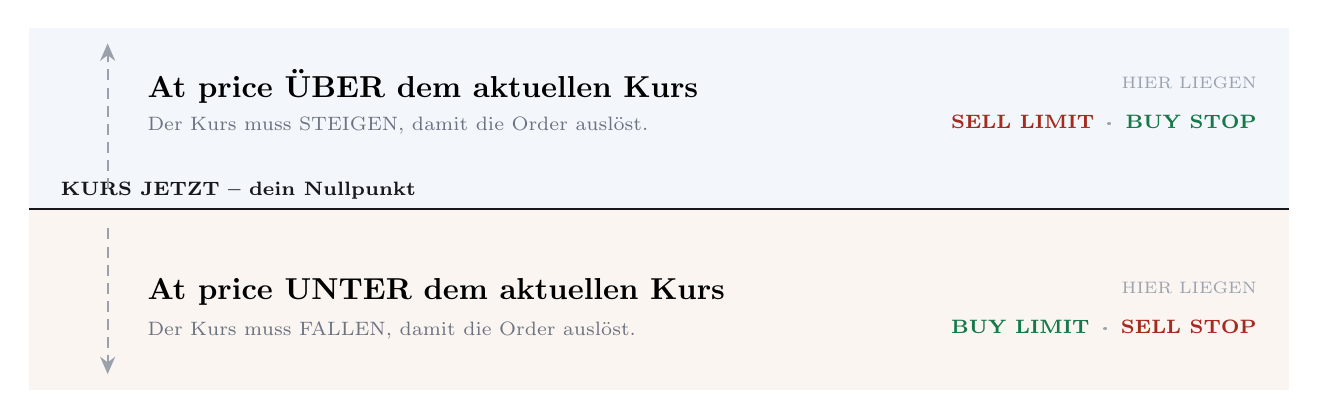
\begin{tikzpicture}[x=1mm,y=1mm,font=\fine]
\fill[tintblue] (0,0) rectangle (160,23);
\fill[tintpeach] (0,-23) rectangle (160,0);
\draw[ink,line width=0.9pt] (0,0) -- (160,0);
\node[anchor=south west,inner sep=0,font=\fine\bfseries,text=ink] at (4,1.2) {KURS JETZT – dein Nullpunkt};
\draw[greya,line width=0.8pt,dash pattern=on 1.4mm off 0.9mm,-{Stealth[length=2.2mm,width=1.9mm]}] (10,2.5) -- (10,21);
\node[anchor=west,inner sep=0,font=\htwo] at (15,15.5) {At price ÜBER dem aktuellen Kurs};
\node[anchor=west,inner sep=0,text=muted] at (15,10.5) {Der Kurs muss STEIGEN, damit die Order auslöst.};
\node[anchor=east,inner sep=0,font=\foot,text=soft] at (156,16) {HIER LIEGEN};
\node[anchor=east,inner sep=0,font=\fine\bfseries] at (156,11) {\textcolor{sell}{SELL LIMIT} {\color{soft}\,·\,} \textcolor{buy}{BUY STOP}};
\draw[greya,line width=0.8pt,dash pattern=on 1.4mm off 0.9mm,-{Stealth[length=2.2mm,width=1.9mm]}] (10,-2.5) -- (10,-21);
\node[anchor=west,inner sep=0,font=\htwo] at (15,-10.5) {At price UNTER dem aktuellen Kurs};
\node[anchor=west,inner sep=0,text=muted] at (15,-15.5) {Der Kurs muss FALLEN, damit die Order auslöst.};
\node[anchor=east,inner sep=0,font=\foot,text=soft] at (156,-10) {HIER LIEGEN};
\node[anchor=east,inner sep=0,font=\fine\bfseries] at (156,-15) {\textcolor{buy}{BUY LIMIT} {\color{soft}\,·\,} \textcolor{sell}{SELL STOP}};
\end{tikzpicture}\par\vspace{5mm}
\noindent\begin{minipage}[t]{84mm}\vspace{0pt}\begin{plain}{\htwo NEW MARKET ORDER}\par\vspace{1.2mm}
{\color{muted}Der linke Reiter: Buy oder Sell \textbf{sofort} zum aktuellen Kurs. Kein At price, kein Warten – ein Klick und die Position ist offen.}\end{plain}\end{minipage}\hfill
\begin{minipage}[t]{84mm}\vspace{0pt}\begin{plain}{\htwo NEW PENDING ORDER}\par\vspace{1.2mm}
{\color{muted}Der rechte Reiter: die Order \textbf{wartet}, bis der Kurs deinen At-price-Wert berührt. Hier stehen die vier Typen aus diesem Guide.}\end{plain}\end{minipage}
\begin{merk}Eine Pending Order ist nichts anderes als eine Market Order \textbf{mit einer Bedingung}. Sie wartet, bis der Kurs deinen At-price-Wert berührt – danach passiert exakt dasselbe wie bei einer Market Order.\end{merk}
\hr
\Htwo{So liest du die Grafiken}
\noindent{\setlength{\tabcolsep}{0pt}\begin{tabular}{@{}p{9mm}@{\hskip 2mm}>{\raggedright\arraybackslash}p{43mm}@{\hskip 6mm}p{9mm}@{\hskip 2mm}>{\raggedright\arraybackslash}p{43mm}@{\hskip 6mm}p{9mm}@{\hskip 2mm}>{\raggedright\arraybackslash}p{43mm}@{}}
\raisebox{-2.2mm}{\begin{tikzpicture}[x=1mm,y=1mm]\useasboundingbox (0,0) rectangle (9,6); \draw[ink,line width=0.8pt] (0,3) -- (9,3);\end{tikzpicture}} & {\htwo Kurs jetzt}\newline{\color{muted}Der aktuelle Kurs, dein Nullpunkt.} & \raisebox{-2.2mm}{\begin{tikzpicture}[x=1mm,y=1mm]\useasboundingbox (0,0) rectangle (9,6); \draw[buy,line width=0.8pt,dash pattern=on 2mm off 1.1mm] (0,3) -- (9,3);\end{tikzpicture}} & {\htwo At-price-Linie}\newline{\color{muted}Dein Wert aus dem Feld „At price“.} & \raisebox{-2.2mm}{\begin{tikzpicture}[x=1mm,y=1mm]\useasboundingbox (0,0) rectangle (9,6); \draw[greya,line width=0.6pt,dash pattern=on 1.2mm off 0.8mm,-{Stealth[length=1.8mm,width=1.5mm]}] (4.5,6) -- (4.5,0);\end{tikzpicture}} & {\htwo Grauer Pfeil}\newline{\color{muted}Weg des Kurses bis zur Auslösung.} \\[4.5mm]
\raisebox{-2.2mm}{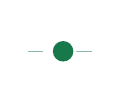
\begin{tikzpicture}[x=1mm,y=1mm]\useasboundingbox (0,0) rectangle (9,6); \draw[buy!50,line width=0.5pt,dash pattern=on 2mm off 1.1mm] (0,3) -- (9,3); \fill[white] (4.5,3) circle (1.7); \fill[buy] (4.5,3) circle (1.3);\end{tikzpicture}} & {\htwo Auslöse-Punkt}\newline{\color{muted}Hier wird dein Buy bzw. Sell ausgeführt.} & \raisebox{-2.2mm}{\begin{tikzpicture}[x=1mm,y=1mm]\useasboundingbox (0,0) rectangle (9,6); \draw[buy,line width=0.85pt,-{Stealth[length=2mm,width=1.7mm]}] (4.5,0) -- (4.5,6);\end{tikzpicture}} & {\htwo Farbiger Pfeil}\newline{\color{muted}So soll der Kurs danach laufen.} & \raisebox{-2.2mm}{\begin{tikzpicture}[x=1mm,y=1mm]\useasboundingbox (0,0) rectangle (9,6); \draw[buy,line width=0.5pt,dash pattern=on 0.6mm off 0.8mm] (0,3) -- (9,3);\end{tikzpicture}} & {\htwo Take-Profit-Linie}\newline{\color{muted}Dein Gewinnziel aus „Set Take-Profit“.} \\[4.5mm]
\raisebox{-2.2mm}{\begin{tikzpicture}[x=1mm,y=1mm]\useasboundingbox (0,0) rectangle (9,6); \draw[buy,line width=0.5pt,dash pattern=on 0.6mm off 0.8mm] (0,6) -- (6,6); \draw[buy,line width=0.7pt,dash pattern=on 2mm off 1.1mm] (0,0) -- (6,0); \draw[buy,line width=0.5pt] (6.5,0) -- (8,0) -- (8,6) -- (6.5,6);\end{tikzpicture}} & {\htwo Gewinn-Klammer}\newline{\color{muted}Von At price bis Take-Profit bist du im Plus.} &  &  &  &  \\[4.5mm]
\end{tabular}}\par\vspace{1.5mm}
{\fine\color{soft}Grün = Buy \,·\, Rot = Sell.}\par
\hr
\Htwo{Zwei Fragen führen zum richtigen Type}
\noindent{\setlength{\tabcolsep}{0pt}\begin{tabular}{@{}l@{\hskip 3mm}c@{\hskip 4mm}c@{}}
 & {\foot\bfseries\color{buy}\ls KAUFEN = BUY} & {\foot\bfseries\color{sell}\ls VERKAUFEN = SELL} \\[1.5mm]
\tikz[baseline=(current bounding box.center)]\node[inner sep=0,text width=42mm,align=left,text=muted]{At price \textbf{ÜBER} dem Kurs}; & \tikz[baseline=(current bounding box.center)]\node[draw=rule,line width=0.4pt,rounded corners=1.5mm,minimum width=62mm,minimum height=13mm,align=center,inner sep=2mm]{{\htwo\color{buy}BUY STOP}\\[0.8mm]{\fine\color{soft}Typ 3 · Ausbruch nach oben kaufen}}; & \tikz[baseline=(current bounding box.center)]\node[draw=rule,line width=0.4pt,rounded corners=1.5mm,minimum width=62mm,minimum height=13mm,align=center,inner sep=2mm]{{\htwo\color{sell}SELL LIMIT}\\[0.8mm]{\fine\color{soft}Typ 2 · teurer verkaufen}}; \\[2.5mm]
\tikz[baseline=(current bounding box.center)]\node[inner sep=0,text width=42mm,align=left,text=muted]{At price \textbf{UNTER} dem Kurs}; & \tikz[baseline=(current bounding box.center)]\node[draw=rule,line width=0.4pt,rounded corners=1.5mm,minimum width=62mm,minimum height=13mm,align=center,inner sep=2mm]{{\htwo\color{buy}BUY LIMIT}\\[0.8mm]{\fine\color{soft}Typ 1 · günstiger kaufen}}; & \tikz[baseline=(current bounding box.center)]\node[draw=rule,line width=0.4pt,rounded corners=1.5mm,minimum width=62mm,minimum height=13mm,align=center,inner sep=2mm]{{\htwo\color{sell}SELL STOP}\\[0.8mm]{\fine\color{soft}Typ 4 · Ausbruch nach unten verkaufen}};
\end{tabular}}
\clearpage

\eyebrow{02 · Die Limit-Typen}
\Hone{Limit = nur zum besseren Kurs}
\lead{Bei Limit liegt dein At-price-Wert immer dort, wo du einen \textbf{günstigeren} Preis bekommst als jetzt. Der Kurs muss erst dorthin laufen – dann löst die Order aus.}

\begin{card}
{\htwo\color{buy}BUY LIMIT}\hspace{2.5mm}{\fine\color{soft}Typ 1}\hfill
{\fine\color{muted}günstiger kaufen \,·\, At price liegt \textbf{UNTER} dem Kurs}\\[1.2mm]
{\color{rule}\rule{\linewidth}{0.4pt}}\\[3mm]
\begin{minipage}[t]{95mm}\vspace{0pt}\hspace{6mm}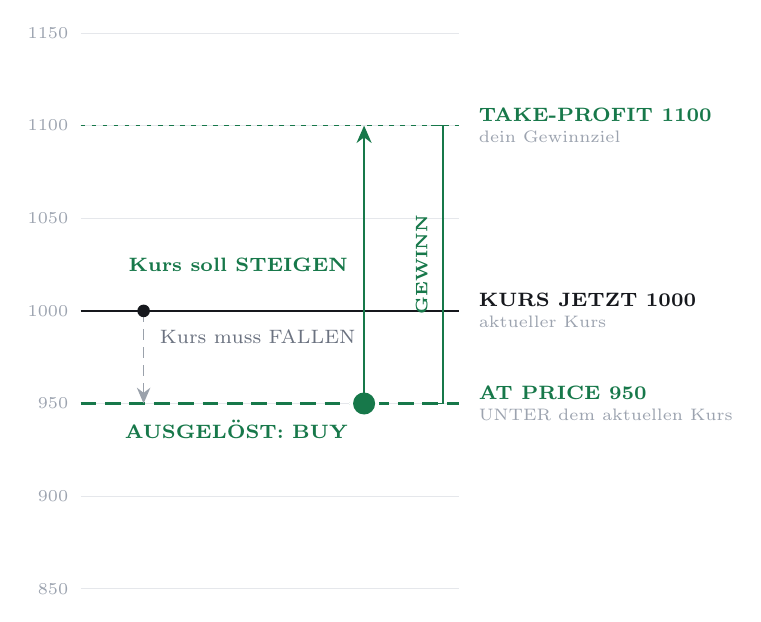
\begin{tikzpicture}[x=1mm,y=1mm,font=\fine,baseline=(current bounding box.north)]
\draw[rule,line width=0.3pt] (0,4.71) -- (48,4.71);
\node[anchor=east,inner sep=0,font=\foot,text=soft] at (-1.5,4.71) {850};
\draw[rule,line width=0.3pt] (0,16.47) -- (48,16.47);
\node[anchor=east,inner sep=0,font=\foot,text=soft] at (-1.5,16.47) {900};
\draw[rule,line width=0.3pt] (0,28.24) -- (48,28.24);
\node[anchor=east,inner sep=0,font=\foot,text=soft] at (-1.5,28.24) {950};
\draw[rule,line width=0.3pt] (0,40.00) -- (48,40.00);
\node[anchor=east,inner sep=0,font=\foot,text=soft] at (-1.5,40.00) {1000};
\draw[rule,line width=0.3pt] (0,51.76) -- (48,51.76);
\node[anchor=east,inner sep=0,font=\foot,text=soft] at (-1.5,51.76) {1050};
\draw[rule,line width=0.3pt] (0,63.53) -- (48,63.53);
\node[anchor=east,inner sep=0,font=\foot,text=soft] at (-1.5,63.53) {1100};
\draw[rule,line width=0.3pt] (0,75.29) -- (48,75.29);
\node[anchor=east,inner sep=0,font=\foot,text=soft] at (-1.5,75.29) {1150};
\draw[buy,line width=0.5pt,dash pattern=on 0.6mm off 0.8mm] (0,63.53) -- (48,63.53);
\draw[ink,line width=0.75pt] (0,40.00) -- (48,40.00);
\draw[buy,line width=0.75pt,dash pattern=on 2mm off 1.1mm] (0,28.24) -- (48,28.24);
\draw[greya,line width=0.6pt,dash pattern=on 1.4mm off 0.9mm,-{Stealth[length=2mm,width=1.7mm]}] (8,40.00) -- (8,28.24);
\fill[ink] (8,40.00) circle (0.8);
\node[anchor=west,inner sep=0,text=muted] at (10,36.70) {Kurs muss FALLEN};
\fill[white] (36,28.24) circle (1.9); \fill[buy] (36,28.24) circle (1.4);
\node[anchor=east,inner sep=0,text=buy,font=\fine\bfseries] at (34,24.94) {AUSGELÖST: BUY};
\draw[buy,line width=0.85pt,-{Stealth[length=2.2mm,width=1.9mm]}] (36,28.24) -- (36,63.53);
\node[anchor=east,inner sep=0,text=buy,font=\fine\bfseries] at (34,45.88) {Kurs soll STEIGEN};
\draw[buy,line width=0.5pt] (44.5,28.24) -- (46,28.24) -- (46,63.53) -- (44.5,63.53);
\node[rotate=90,inner sep=0,text=buy,font=\foot\bfseries] at (43.3,45.88) {GEWINN};
\node[anchor=south west,inner sep=0,text=buy,font=\fine\bfseries] at (50.5,64.03) {TAKE-PROFIT 1100};
\node[anchor=north west,inner sep=0,text=soft,font=\foot] at (50.5,62.93) {dein Gewinnziel};
\node[anchor=south west,inner sep=0,text=ink,font=\fine\bfseries] at (50.5,40.50) {KURS JETZT 1000};
\node[anchor=north west,inner sep=0,text=soft,font=\foot] at (50.5,39.40) {aktueller Kurs};
\node[anchor=south west,inner sep=0,text=buy,font=\fine\bfseries] at (50.5,28.74) {AT PRICE 950};
\node[anchor=north west,inner sep=0,text=soft,font=\foot] at (50.5,27.64) {UNTER dem aktuellen Kurs};
\end{tikzpicture}\end{minipage}\hfill
\begin{minipage}[t]{63mm}\vspace{0pt}\raggedright
\begin{stepsx}{buy}
\item Bei \textbf{At price} einen Wert \textbf{UNTER} dem aktuellen Kurs eintragen – hier \textbf{950}
\item Warten: der Kurs muss auf \textbf{950} fallen
\item Auslösung: dein \textbf{BUY} wird ausgeführt – die Position ist offen
\end{stepsx}
\begin{note}{buy}{DANACH}Der Kurs soll \textbf{steigen}. Dein Take-Profit liegt bei \textbf{1100}.\end{note}
{\fine\color{soft}Typisch: einen Rücksetzer abwarten und tiefer einsteigen.}
\end{minipage}
\end{card}

\begin{card}
{\htwo\color{sell}SELL LIMIT}\hspace{2.5mm}{\fine\color{soft}Typ 2}\hfill
{\fine\color{muted}teurer verkaufen \,·\, At price liegt \textbf{ÜBER} dem Kurs}\\[1.2mm]
{\color{rule}\rule{\linewidth}{0.4pt}}\\[3mm]
\begin{minipage}[t]{95mm}\vspace{0pt}\hspace{6mm}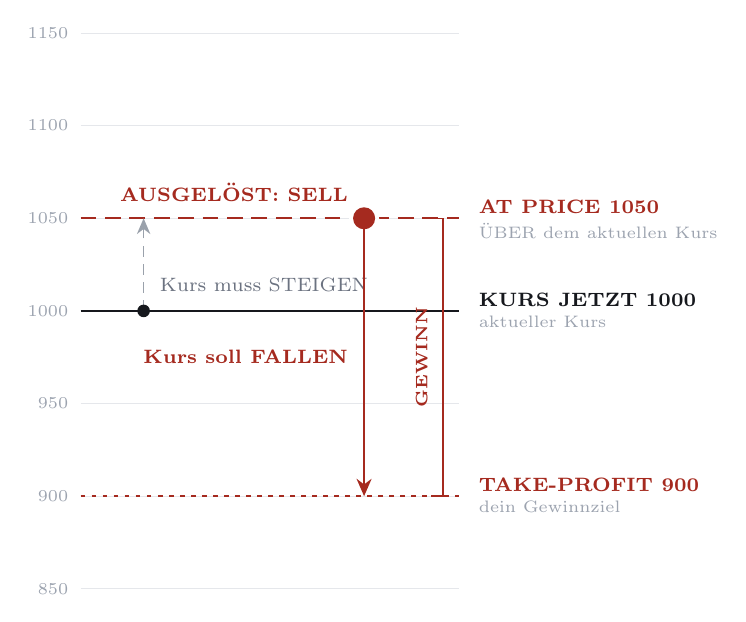
\begin{tikzpicture}[x=1mm,y=1mm,font=\fine,baseline=(current bounding box.north)]
\draw[rule,line width=0.3pt] (0,4.71) -- (48,4.71);
\node[anchor=east,inner sep=0,font=\foot,text=soft] at (-1.5,4.71) {850};
\draw[rule,line width=0.3pt] (0,16.47) -- (48,16.47);
\node[anchor=east,inner sep=0,font=\foot,text=soft] at (-1.5,16.47) {900};
\draw[rule,line width=0.3pt] (0,28.24) -- (48,28.24);
\node[anchor=east,inner sep=0,font=\foot,text=soft] at (-1.5,28.24) {950};
\draw[rule,line width=0.3pt] (0,40.00) -- (48,40.00);
\node[anchor=east,inner sep=0,font=\foot,text=soft] at (-1.5,40.00) {1000};
\draw[rule,line width=0.3pt] (0,51.76) -- (48,51.76);
\node[anchor=east,inner sep=0,font=\foot,text=soft] at (-1.5,51.76) {1050};
\draw[rule,line width=0.3pt] (0,63.53) -- (48,63.53);
\node[anchor=east,inner sep=0,font=\foot,text=soft] at (-1.5,63.53) {1100};
\draw[rule,line width=0.3pt] (0,75.29) -- (48,75.29);
\node[anchor=east,inner sep=0,font=\foot,text=soft] at (-1.5,75.29) {1150};
\draw[sell,line width=0.5pt,dash pattern=on 0.6mm off 0.8mm] (0,16.47) -- (48,16.47);
\draw[ink,line width=0.75pt] (0,40.00) -- (48,40.00);
\draw[sell,line width=0.75pt,dash pattern=on 2mm off 1.1mm] (0,51.76) -- (48,51.76);
\draw[greya,line width=0.6pt,dash pattern=on 1.4mm off 0.9mm,-{Stealth[length=2mm,width=1.7mm]}] (8,40.00) -- (8,51.76);
\fill[ink] (8,40.00) circle (0.8);
\node[anchor=west,inner sep=0,text=muted] at (10,43.30) {Kurs muss STEIGEN};
\fill[white] (36,51.76) circle (1.9); \fill[sell] (36,51.76) circle (1.4);
\node[anchor=east,inner sep=0,text=sell,font=\fine\bfseries] at (34,55.06) {AUSGELÖST: SELL};
\draw[sell,line width=0.85pt,-{Stealth[length=2.2mm,width=1.9mm]}] (36,51.76) -- (36,16.47);
\node[anchor=east,inner sep=0,text=sell,font=\fine\bfseries] at (34,34.12) {Kurs soll FALLEN};
\draw[sell,line width=0.5pt] (44.5,51.76) -- (46,51.76) -- (46,16.47) -- (44.5,16.47);
\node[rotate=90,inner sep=0,text=sell,font=\foot\bfseries] at (43.3,34.12) {GEWINN};
\node[anchor=south west,inner sep=0,text=sell,font=\fine\bfseries] at (50.5,16.97) {TAKE-PROFIT 900};
\node[anchor=north west,inner sep=0,text=soft,font=\foot] at (50.5,15.87) {dein Gewinnziel};
\node[anchor=south west,inner sep=0,text=ink,font=\fine\bfseries] at (50.5,40.50) {KURS JETZT 1000};
\node[anchor=north west,inner sep=0,text=soft,font=\foot] at (50.5,39.40) {aktueller Kurs};
\node[anchor=south west,inner sep=0,text=sell,font=\fine\bfseries] at (50.5,52.26) {AT PRICE 1050};
\node[anchor=north west,inner sep=0,text=soft,font=\foot] at (50.5,51.16) {ÜBER dem aktuellen Kurs};
\end{tikzpicture}\end{minipage}\hfill
\begin{minipage}[t]{63mm}\vspace{0pt}\raggedright
\begin{stepsx}{sell}
\item Bei \textbf{At price} einen Wert \textbf{ÜBER} dem aktuellen Kurs eintragen – hier \textbf{1050}
\item Warten: der Kurs muss auf \textbf{1050} steigen
\item Auslösung: dein \textbf{SELL} wird ausgeführt – die Position ist offen
\end{stepsx}
\begin{note}{sell}{DANACH}Der Kurs soll \textbf{fallen}. Dein Take-Profit liegt bei \textbf{900}.\end{note}
{\fine\color{soft}Typisch: einen Anstieg abwarten und oben verkaufen.}
\end{minipage}
\end{card}
\clearpage

\eyebrow{03 · Die Stop-Typen}
\Hone{Stop = erst bei Bewegung}
\lead{Bei Stop liegt dein At-price-Wert auf der \textbf{ungünstigeren} Seite. Die Order löst aus, sobald der Kurs durch den Wert bricht – du steigst also erst ein, wenn die Bewegung da ist.}

\begin{card}
{\htwo\color{buy}BUY STOP}\hspace{2.5mm}{\fine\color{soft}Typ 3}\hfill
{\fine\color{muted}Ausbruch nach oben kaufen \,·\, At price liegt \textbf{ÜBER} dem Kurs}\\[1.2mm]
{\color{rule}\rule{\linewidth}{0.4pt}}\\[3mm]
\begin{minipage}[t]{95mm}\vspace{0pt}\hspace{6mm}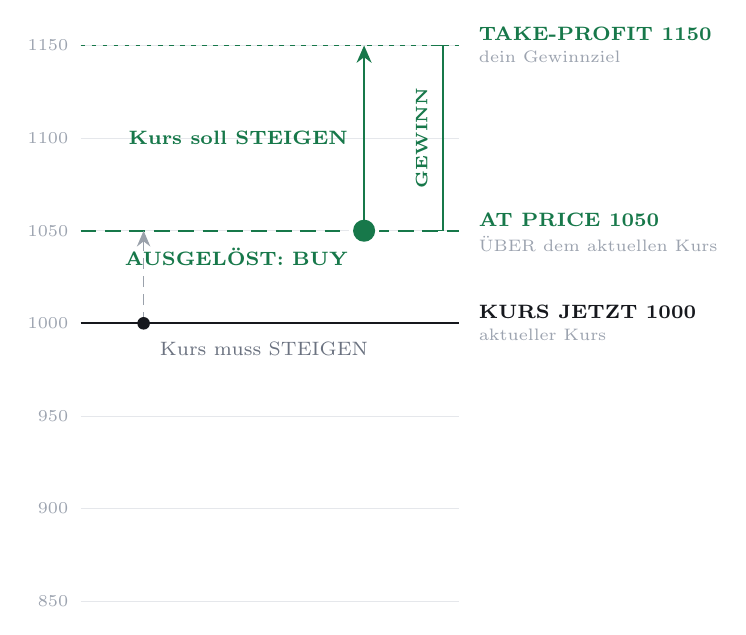
\begin{tikzpicture}[x=1mm,y=1mm,font=\fine,baseline=(current bounding box.north)]
\draw[rule,line width=0.3pt] (0,4.71) -- (48,4.71);
\node[anchor=east,inner sep=0,font=\foot,text=soft] at (-1.5,4.71) {850};
\draw[rule,line width=0.3pt] (0,16.47) -- (48,16.47);
\node[anchor=east,inner sep=0,font=\foot,text=soft] at (-1.5,16.47) {900};
\draw[rule,line width=0.3pt] (0,28.24) -- (48,28.24);
\node[anchor=east,inner sep=0,font=\foot,text=soft] at (-1.5,28.24) {950};
\draw[rule,line width=0.3pt] (0,40.00) -- (48,40.00);
\node[anchor=east,inner sep=0,font=\foot,text=soft] at (-1.5,40.00) {1000};
\draw[rule,line width=0.3pt] (0,51.76) -- (48,51.76);
\node[anchor=east,inner sep=0,font=\foot,text=soft] at (-1.5,51.76) {1050};
\draw[rule,line width=0.3pt] (0,63.53) -- (48,63.53);
\node[anchor=east,inner sep=0,font=\foot,text=soft] at (-1.5,63.53) {1100};
\draw[rule,line width=0.3pt] (0,75.29) -- (48,75.29);
\node[anchor=east,inner sep=0,font=\foot,text=soft] at (-1.5,75.29) {1150};
\draw[buy,line width=0.5pt,dash pattern=on 0.6mm off 0.8mm] (0,75.29) -- (48,75.29);
\draw[ink,line width=0.75pt] (0,40.00) -- (48,40.00);
\draw[buy,line width=0.75pt,dash pattern=on 2mm off 1.1mm] (0,51.76) -- (48,51.76);
\draw[greya,line width=0.6pt,dash pattern=on 1.4mm off 0.9mm,-{Stealth[length=2mm,width=1.7mm]}] (8,40.00) -- (8,51.76);
\fill[ink] (8,40.00) circle (0.8);
\node[anchor=west,inner sep=0,text=muted] at (10,36.70) {Kurs muss STEIGEN};
\fill[white] (36,51.76) circle (1.9); \fill[buy] (36,51.76) circle (1.4);
\node[anchor=east,inner sep=0,text=buy,font=\fine\bfseries] at (34,48.46) {AUSGELÖST: BUY};
\draw[buy,line width=0.85pt,-{Stealth[length=2.2mm,width=1.9mm]}] (36,51.76) -- (36,75.29);
\node[anchor=east,inner sep=0,text=buy,font=\fine\bfseries] at (34,63.53) {Kurs soll STEIGEN};
\draw[buy,line width=0.5pt] (44.5,51.76) -- (46,51.76) -- (46,75.29) -- (44.5,75.29);
\node[rotate=90,inner sep=0,text=buy,font=\foot\bfseries] at (43.3,63.53) {GEWINN};
\node[anchor=south west,inner sep=0,text=buy,font=\fine\bfseries] at (50.5,75.79) {TAKE-PROFIT 1150};
\node[anchor=north west,inner sep=0,text=soft,font=\foot] at (50.5,74.69) {dein Gewinnziel};
\node[anchor=south west,inner sep=0,text=ink,font=\fine\bfseries] at (50.5,40.50) {KURS JETZT 1000};
\node[anchor=north west,inner sep=0,text=soft,font=\foot] at (50.5,39.40) {aktueller Kurs};
\node[anchor=south west,inner sep=0,text=buy,font=\fine\bfseries] at (50.5,52.26) {AT PRICE 1050};
\node[anchor=north west,inner sep=0,text=soft,font=\foot] at (50.5,51.16) {ÜBER dem aktuellen Kurs};
\end{tikzpicture}\end{minipage}\hfill
\begin{minipage}[t]{63mm}\vspace{0pt}\raggedright
\begin{stepsx}{buy}
\item Bei \textbf{At price} einen Wert \textbf{ÜBER} dem aktuellen Kurs eintragen – hier \textbf{1050}
\item Der Kurs bricht nach \textbf{oben} durch \textbf{1050}
\item Auslösung: dein \textbf{BUY} wird ausgeführt – die Position ist offen
\end{stepsx}
\begin{note}{buy}{DANACH}Der Kurs soll \textbf{steigen}. Dein Take-Profit liegt bei \textbf{1150}.\end{note}
{\fine\color{soft}Typisch: erst kaufen, wenn der Kurs nach oben ausbricht.}
\end{minipage}
\end{card}

\begin{card}
{\htwo\color{sell}SELL STOP}\hspace{2.5mm}{\fine\color{soft}Typ 4}\hfill
{\fine\color{muted}Ausbruch nach unten verkaufen \,·\, At price liegt \textbf{UNTER} dem Kurs}\\[1.2mm]
{\color{rule}\rule{\linewidth}{0.4pt}}\\[3mm]
\begin{minipage}[t]{95mm}\vspace{0pt}\hspace{6mm}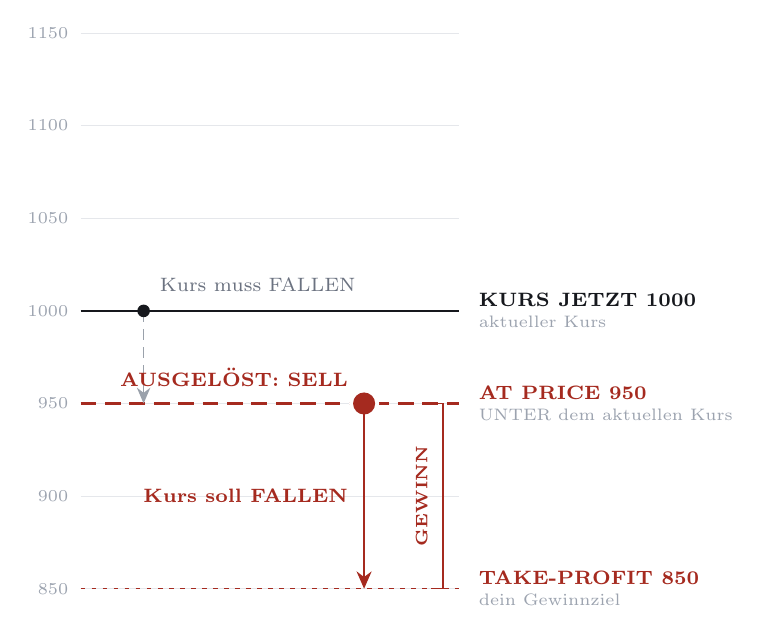
\begin{tikzpicture}[x=1mm,y=1mm,font=\fine,baseline=(current bounding box.north)]
\draw[rule,line width=0.3pt] (0,4.71) -- (48,4.71);
\node[anchor=east,inner sep=0,font=\foot,text=soft] at (-1.5,4.71) {850};
\draw[rule,line width=0.3pt] (0,16.47) -- (48,16.47);
\node[anchor=east,inner sep=0,font=\foot,text=soft] at (-1.5,16.47) {900};
\draw[rule,line width=0.3pt] (0,28.24) -- (48,28.24);
\node[anchor=east,inner sep=0,font=\foot,text=soft] at (-1.5,28.24) {950};
\draw[rule,line width=0.3pt] (0,40.00) -- (48,40.00);
\node[anchor=east,inner sep=0,font=\foot,text=soft] at (-1.5,40.00) {1000};
\draw[rule,line width=0.3pt] (0,51.76) -- (48,51.76);
\node[anchor=east,inner sep=0,font=\foot,text=soft] at (-1.5,51.76) {1050};
\draw[rule,line width=0.3pt] (0,63.53) -- (48,63.53);
\node[anchor=east,inner sep=0,font=\foot,text=soft] at (-1.5,63.53) {1100};
\draw[rule,line width=0.3pt] (0,75.29) -- (48,75.29);
\node[anchor=east,inner sep=0,font=\foot,text=soft] at (-1.5,75.29) {1150};
\draw[sell,line width=0.5pt,dash pattern=on 0.6mm off 0.8mm] (0,4.71) -- (48,4.71);
\draw[ink,line width=0.75pt] (0,40.00) -- (48,40.00);
\draw[sell,line width=0.75pt,dash pattern=on 2mm off 1.1mm] (0,28.24) -- (48,28.24);
\draw[greya,line width=0.6pt,dash pattern=on 1.4mm off 0.9mm,-{Stealth[length=2mm,width=1.7mm]}] (8,40.00) -- (8,28.24);
\fill[ink] (8,40.00) circle (0.8);
\node[anchor=west,inner sep=0,text=muted] at (10,43.30) {Kurs muss FALLEN};
\fill[white] (36,28.24) circle (1.9); \fill[sell] (36,28.24) circle (1.4);
\node[anchor=east,inner sep=0,text=sell,font=\fine\bfseries] at (34,31.54) {AUSGELÖST: SELL};
\draw[sell,line width=0.85pt,-{Stealth[length=2.2mm,width=1.9mm]}] (36,28.24) -- (36,4.71);
\node[anchor=east,inner sep=0,text=sell,font=\fine\bfseries] at (34,16.47) {Kurs soll FALLEN};
\draw[sell,line width=0.5pt] (44.5,28.24) -- (46,28.24) -- (46,4.71) -- (44.5,4.71);
\node[rotate=90,inner sep=0,text=sell,font=\foot\bfseries] at (43.3,16.47) {GEWINN};
\node[anchor=south west,inner sep=0,text=sell,font=\fine\bfseries] at (50.5,5.21) {TAKE-PROFIT 850};
\node[anchor=north west,inner sep=0,text=soft,font=\foot] at (50.5,4.11) {dein Gewinnziel};
\node[anchor=south west,inner sep=0,text=ink,font=\fine\bfseries] at (50.5,40.50) {KURS JETZT 1000};
\node[anchor=north west,inner sep=0,text=soft,font=\foot] at (50.5,39.40) {aktueller Kurs};
\node[anchor=south west,inner sep=0,text=sell,font=\fine\bfseries] at (50.5,28.74) {AT PRICE 950};
\node[anchor=north west,inner sep=0,text=soft,font=\foot] at (50.5,27.64) {UNTER dem aktuellen Kurs};
\end{tikzpicture}\end{minipage}\hfill
\begin{minipage}[t]{63mm}\vspace{0pt}\raggedright
\begin{stepsx}{sell}
\item Bei \textbf{At price} einen Wert \textbf{UNTER} dem aktuellen Kurs eintragen – hier \textbf{950}
\item Der Kurs bricht nach \textbf{unten} durch \textbf{950}
\item Auslösung: dein \textbf{SELL} wird ausgeführt – die Position ist offen
\end{stepsx}
\begin{note}{sell}{DANACH}Der Kurs soll \textbf{fallen}. Dein Take-Profit liegt bei \textbf{850}.\end{note}
{\fine\color{soft}Typisch: erst verkaufen, wenn der Kurs nach unten durchbricht.}
\end{minipage}
\end{card}
\clearpage

\eyebrow{04 · Spickzettel}
\Hone{Alle vier Typen auf einer Leiter}
\lead{Oben die beiden At-price-Werte über dem Kurs, unten die beiden darunter. Grauer Pfeil: der Weg bis zur Auslösung. Farbiger Pfeil: die Richtung danach.}
\vspace{5mm}\par\hspace{9mm}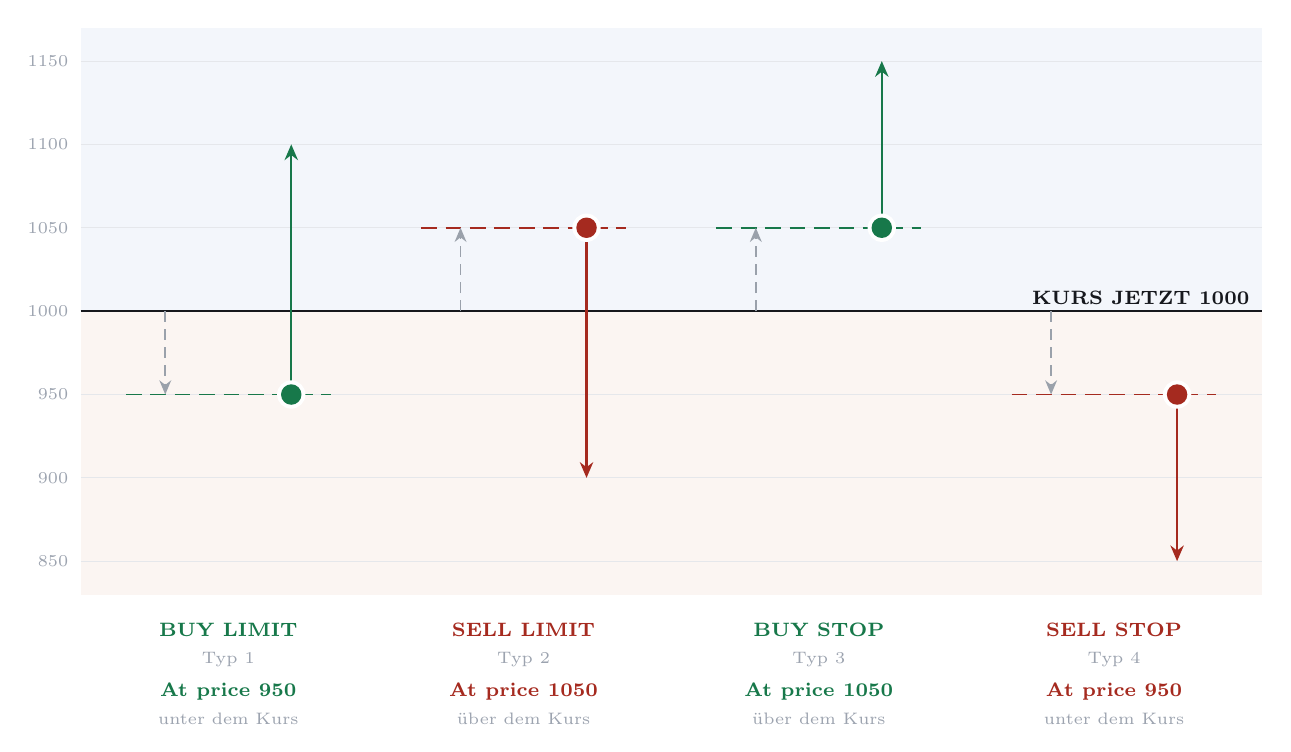
\begin{tikzpicture}[x=1mm,y=1mm,font=\fine]
\fill[tintblue] (0,36.00) rectangle (150,72);
\fill[tintpeach] (0,0) rectangle (150,36.00);
\draw[rule,line width=0.3pt] (0,4.24) -- (150,4.24);
\node[anchor=east,inner sep=0,font=\foot,text=soft] at (-1.5,4.24) {850};
\draw[rule,line width=0.3pt] (0,14.82) -- (150,14.82);
\node[anchor=east,inner sep=0,font=\foot,text=soft] at (-1.5,14.82) {900};
\draw[rule,line width=0.3pt] (0,25.41) -- (150,25.41);
\node[anchor=east,inner sep=0,font=\foot,text=soft] at (-1.5,25.41) {950};
\draw[rule,line width=0.3pt] (0,36.00) -- (150,36.00);
\node[anchor=east,inner sep=0,font=\foot,text=soft] at (-1.5,36.00) {1000};
\draw[rule,line width=0.3pt] (0,46.59) -- (150,46.59);
\node[anchor=east,inner sep=0,font=\foot,text=soft] at (-1.5,46.59) {1050};
\draw[rule,line width=0.3pt] (0,57.18) -- (150,57.18);
\node[anchor=east,inner sep=0,font=\foot,text=soft] at (-1.5,57.18) {1100};
\draw[rule,line width=0.3pt] (0,67.76) -- (150,67.76);
\node[anchor=east,inner sep=0,font=\foot,text=soft] at (-1.5,67.76) {1150};
\draw[ink,line width=0.8pt] (0,36.00) -- (150,36.00);
\node[anchor=south east,inner sep=0,font=\fine\bfseries,text=ink] at (148.5,36.80) {KURS JETZT 1000};
\draw[buy,line width=0.7pt,dash pattern=on 2mm off 1.1mm] (5.75,25.41) -- (31.75,25.41);
\draw[greya,line width=0.6pt,dash pattern=on 1.4mm off 0.9mm,-{Stealth[length=1.8mm,width=1.5mm]}] (10.75,36.00) -- (10.75,25.41);
\draw[buy,line width=0.8pt,-{Stealth[length=2mm,width=1.7mm]}] (26.75,25.41) -- (26.75,57.18);
\fill[white] (26.75,25.41) circle (1.8); \fill[buy] (26.75,25.41) circle (1.3);
\node[anchor=north,inner sep=0,font=\fine\bfseries,text=buy] at (18.75,-3.5) {BUY LIMIT};
\node[anchor=north,inner sep=0,font=\foot,text=soft] at (18.75,-7.2) {Typ 1};
\node[anchor=north,inner sep=0,font=\fine\bfseries,text=buy] at (18.75,-11.2) {At price 950};
\node[anchor=north,inner sep=0,font=\foot,text=soft] at (18.75,-14.9) {unter dem Kurs};
\draw[sell,line width=0.7pt,dash pattern=on 2mm off 1.1mm] (43.25,46.59) -- (69.25,46.59);
\draw[greya,line width=0.6pt,dash pattern=on 1.4mm off 0.9mm,-{Stealth[length=1.8mm,width=1.5mm]}] (48.25,36.00) -- (48.25,46.59);
\draw[sell,line width=0.8pt,-{Stealth[length=2mm,width=1.7mm]}] (64.25,46.59) -- (64.25,14.82);
\fill[white] (64.25,46.59) circle (1.8); \fill[sell] (64.25,46.59) circle (1.3);
\node[anchor=north,inner sep=0,font=\fine\bfseries,text=sell] at (56.25,-3.5) {SELL LIMIT};
\node[anchor=north,inner sep=0,font=\foot,text=soft] at (56.25,-7.2) {Typ 2};
\node[anchor=north,inner sep=0,font=\fine\bfseries,text=sell] at (56.25,-11.2) {At price 1050};
\node[anchor=north,inner sep=0,font=\foot,text=soft] at (56.25,-14.9) {über dem Kurs};
\draw[buy,line width=0.7pt,dash pattern=on 2mm off 1.1mm] (80.75,46.59) -- (106.75,46.59);
\draw[greya,line width=0.6pt,dash pattern=on 1.4mm off 0.9mm,-{Stealth[length=1.8mm,width=1.5mm]}] (85.75,36.00) -- (85.75,46.59);
\draw[buy,line width=0.8pt,-{Stealth[length=2mm,width=1.7mm]}] (101.75,46.59) -- (101.75,67.76);
\fill[white] (101.75,46.59) circle (1.8); \fill[buy] (101.75,46.59) circle (1.3);
\node[anchor=north,inner sep=0,font=\fine\bfseries,text=buy] at (93.75,-3.5) {BUY STOP};
\node[anchor=north,inner sep=0,font=\foot,text=soft] at (93.75,-7.2) {Typ 3};
\node[anchor=north,inner sep=0,font=\fine\bfseries,text=buy] at (93.75,-11.2) {At price 1050};
\node[anchor=north,inner sep=0,font=\foot,text=soft] at (93.75,-14.9) {über dem Kurs};
\draw[sell,line width=0.7pt,dash pattern=on 2mm off 1.1mm] (118.25,25.41) -- (144.25,25.41);
\draw[greya,line width=0.6pt,dash pattern=on 1.4mm off 0.9mm,-{Stealth[length=1.8mm,width=1.5mm]}] (123.25,36.00) -- (123.25,25.41);
\draw[sell,line width=0.8pt,-{Stealth[length=2mm,width=1.7mm]}] (139.25,25.41) -- (139.25,4.24);
\fill[white] (139.25,25.41) circle (1.8); \fill[sell] (139.25,25.41) circle (1.3);
\node[anchor=north,inner sep=0,font=\fine\bfseries,text=sell] at (131.25,-3.5) {SELL STOP};
\node[anchor=north,inner sep=0,font=\foot,text=soft] at (131.25,-7.2) {Typ 4};
\node[anchor=north,inner sep=0,font=\fine\bfseries,text=sell] at (131.25,-11.2) {At price 950};
\node[anchor=north,inner sep=0,font=\foot,text=soft] at (131.25,-14.9) {unter dem Kurs};
\end{tikzpicture}\par\vspace{7mm}
\begin{tabularx}{\textwidth}{@{}p{34mm}p{28mm}p{46mm}>{\raggedright\arraybackslash}X@{}}
\hd{Type} & \hd{At price liegt} & \hd{Löst aus, wenn …} & \hd{Danach soll …} \\ \midrule \addlinespace[1.5mm]
\textcolor{buy}{\bfseries BUY LIMIT} \mbox{\foot\color{soft}Typ 1} & unter dem Kurs & der Kurs auf \textbf{950} fallen & der Kurs steigen → Take-Profit \textbf{1100} \\ \addlinespace[2.2mm]
\textcolor{sell}{\bfseries SELL LIMIT} \mbox{\foot\color{soft}Typ 2} & über dem Kurs & der Kurs auf \textbf{1050} steigen & der Kurs fallen → Take-Profit \textbf{900} \\ \addlinespace[2.2mm]
\textcolor{buy}{\bfseries BUY STOP} \mbox{\foot\color{soft}Typ 3} & über dem Kurs & der Kurs auf \textbf{1050} steigen & der Kurs steigen → Take-Profit \textbf{1150} \\ \addlinespace[2.2mm]
\textcolor{sell}{\bfseries SELL STOP} \mbox{\foot\color{soft}Typ 4} & unter dem Kurs & der Kurs auf \textbf{950} fallen & der Kurs fallen → Take-Profit \textbf{850} \\ \addlinespace[2.2mm]
\end{tabularx}
\begin{merk}\textbf{Zwei Faustregeln.} 1) Erst die Richtung (Buy oder Sell), dann der Ort (At price über oder unter dem Kurs) – daraus ergibt sich der Type von selbst. 2) Limit heißt geduldig auf den besseren Kurs warten, Stop heißt auf Bewegung reagieren.\end{merk}
\clearpage

\eyebrow{05 · In der Plattform}
\Hone{So sieht es im Fenster „New Order“ aus}
\lead{Links das Fenster mit Beispielzahlen, rechts die fünf Stellen, auf die es ankommt. Alles andere kannst du fürs Erste ignorieren.}
\vspace{5mm}\par
\noindent\begin{minipage}[t]{78mm}\vspace{0pt}\begin{tikzpicture}[x=1mm,y=1mm,font=\wfont]
\begin{scope} \clip[rounded corners=2mm] (0,0) rectangle (78.0,96.0);
\fill[wbg] (0,0) rectangle (78.0,96.0); \fill[whead] (0,89.0) rectangle (78.0,96.0); \end{scope}
\draw[wborder,line width=0.4pt,rounded corners=2mm] (0,0) rectangle (78.0,96.0);
\node[text=white,font=\wfont\bfseries] at (39.0,92.5) {NEW ORDER};
\node[text=wmuted] at (74.5,92.5) {×};
\draw[wborder,fill=wfield,rounded corners=1mm] (3,81) rectangle (38.5,87);
\node[text=wtabtext] at (20.75,84) {New Market Order};
\fill[waccent,rounded corners=1mm] (39.5,81) rectangle (75,87);
\node[text=white,font=\wfont\bfseries] at (58.7,84) {New Pending Order};
\node[circle,fill=white,text=wbg,font=\bfseries\fontsize{5.5}{6}\selectfont,inner sep=0,minimum size=2.9mm] at (44,84) {1};
\node[anchor=west,inner sep=0,text=wmuted,font=\wsmall] at (3,78) {Symbol};
\draw[wborder,line width=0.4pt,fill=wfield,rounded corners=1mm] (3,70) rectangle (38.5,76);
\node[anchor=west,inner sep=0,text=wtext] at (5,73) {Instrument XY};
\fill[wmuted] (34.5,73.6) -- (36.5,73.6) -- (35.5,72.3) -- cycle;
\node[anchor=west,inner sep=0,text=wmuted,font=\wsmall] at (44.0,78) {Type};
\node[circle,fill=white,text=wbg,font=\bfseries\fontsize{5.5}{6}\selectfont,inner sep=0,minimum size=2.9mm] at (41.0,78) {2};
\draw[wmark,line width=0.6pt,fill=wfield,rounded corners=1mm] (39.5,70) rectangle (75.0,76);
\node[anchor=west,inner sep=0,text=wtext] at (41.5,73) {Buy Limit};
\fill[wmuted] (71.0,73.6) -- (73.0,73.6) -- (72.0,72.3) -- cycle;
\node[anchor=west,inner sep=0,text=wmuted,font=\wsmall] at (3,66) {Volume};
\draw[wborder,line width=0.4pt,fill=wfield,rounded corners=1mm] (3,58) rectangle (38.5,64);
\node[anchor=west,inner sep=0,text=wtext] at (5,61) {1};
\node[anchor=east,inner sep=0,text=wmuted,font=\wsmall] at (36.5,61) {+\,−};
\node[anchor=west,inner sep=0,text=wmuted,font=\wsmall] at (44.0,66) {At price};
\node[circle,fill=white,text=wbg,font=\bfseries\fontsize{5.5}{6}\selectfont,inner sep=0,minimum size=2.9mm] at (41.0,66) {3};
\draw[wmark,line width=0.6pt,fill=wfield,rounded corners=1mm] (39.5,58) rectangle (75.0,64);
\node[anchor=west,inner sep=0,text=wtext] at (41.5,61) {950};
\node[anchor=east,inner sep=0,text=wmuted,font=\wsmall] at (73.0,61) {+\,−};
\fill[wchart,rounded corners=1mm] (3,34) rectangle (56,55.5);
\fill[wred,opacity=0.8] (5.50,44.50) rectangle (6.40,46.70);
\fill[wred,opacity=0.8] (7.35,44.20) rectangle (8.25,49.04);
\fill[wred,opacity=0.8] (9.20,43.90) rectangle (10.10,48.17);
\fill[wred,opacity=0.8] (11.05,43.60) rectangle (11.95,47.31);
\fill[wred,opacity=0.8] (12.90,43.30) rectangle (13.80,46.44);
\fill[wred,opacity=0.8] (14.75,43.00) rectangle (15.65,45.58);
\fill[wred,opacity=0.8] (16.60,42.70) rectangle (17.50,47.91);
\fill[wred,opacity=0.8] (18.45,42.40) rectangle (19.35,47.05);
\fill[wred,opacity=0.8] (20.30,42.10) rectangle (21.20,46.18);
\fill[wred,opacity=0.8] (22.15,41.80) rectangle (23.05,45.32);
\fill[wred,opacity=0.8] (24.00,41.50) rectangle (24.90,44.45);
\fill[wred,opacity=0.8] (25.85,41.20) rectangle (26.75,43.59);
\fill[wred,opacity=0.8] (27.70,40.90) rectangle (28.60,45.92);
\fill[wgreen,opacity=0.95] (29.55,41.00) rectangle (30.45,45.46);
\fill[wgreen,opacity=0.95] (31.40,41.45) rectangle (32.30,45.34);
\fill[wgreen,opacity=0.95] (33.25,41.90) rectangle (34.15,45.23);
\fill[wgreen,opacity=0.95] (35.10,42.35) rectangle (36.00,45.11);
\fill[wgreen,opacity=0.95] (36.95,42.80) rectangle (37.85,45.00);
\fill[wgreen,opacity=0.95] (38.80,43.25) rectangle (39.70,48.09);
\fill[wgreen,opacity=0.95] (40.65,43.70) rectangle (41.55,47.97);
\fill[wgreen,opacity=0.95] (42.50,44.15) rectangle (43.40,47.86);
\fill[wgreen,opacity=0.95] (44.35,44.60) rectangle (45.25,47.74);
\fill[wgreen,opacity=0.95] (46.20,45.05) rectangle (47.10,47.63);
\fill[wgreen,opacity=0.95] (48.05,45.50) rectangle (48.95,50.71);
\fill[wgreen,opacity=0.95] (49.90,45.95) rectangle (50.80,50.60);
\fill[wgreen,opacity=0.95] (51.75,46.40) rectangle (52.65,50.48);
\fill[wred] (10.5,51.5) circle (0.7); \fill[wpill,rounded corners=0.6mm] (12,49.7) rectangle (21.5,53.3); \node[text=wtext,font=\wsmall] at (16.75,51.5) {1000};
\fill[wgreen] (30,37.8) circle (0.7); \fill[wpill,rounded corners=0.6mm] (20,36) rectangle (29,39.6); \node[text=wtext,font=\wsmall] at (24.5,37.8) {950};
\fill[wgreen] (50.5,50.5) -- (53,50.5) -- (51.75,52.5) -- cycle;
\fill[wtog,rounded corners=1.2mm] (3,29.3) rectangle (7.8,31.7);
\fill[wknob] (4.2,30.5) circle (0.85);
\node[anchor=west,inner sep=0,text=wtabtext] at (9.2,30.5) {Set Stop-Loss};
\draw[wborder,line width=0.4pt,fill=wfield,rounded corners=1mm] (3,21) rectangle (38.5,27); \node[anchor=west,inner sep=0,text=wdim] at (5,24) {0}; \node[anchor=east,inner sep=0,text=wmuted,font=\wsmall] at (36.5,24) {+\,−};
\fill[wgreen,rounded corners=1.2mm] (39.5,29.3) rectangle (44.3,31.7);
\fill[white] (43.1,30.5) circle (0.85);
\node[anchor=west,inner sep=0,text=wtabtext] at (50.2,30.5) {Set Take-Profit};
\node[circle,fill=white,text=wbg,font=\bfseries\fontsize{5.5}{6}\selectfont,inner sep=0,minimum size=2.9mm] at (47.2,30.5) {4};
\draw[wmark,line width=0.6pt,fill=wfield,rounded corners=1mm] (39.5,21) rectangle (75,27); \node[anchor=west,inner sep=0,text=wtext] at (41.5,24) {1100}; \node[anchor=east,inner sep=0,text=wmuted,font=\wsmall] at (73,24) {+\,−};
\node[anchor=west,inner sep=0,text=wmuted,font=\wsmall] at (39.5,18) {Estimated Profit: \textcolor{wgreen}{\bfseries 150\,€}};
\fill[wgreen,rounded corners=1.2mm] (3,6) rectangle (75,13.5);
\node[text=white,font=\wfont\bfseries] at (41,9.75) {Place pending order};
\node[circle,fill=wbadge,text=white,font=\bfseries\fontsize{5.5}{6}\selectfont,inner sep=0,minimum size=2.9mm] at (26.5,9.75) {5};
\end{tikzpicture}\end{minipage}\hfill
\begin{minipage}[t]{88mm}\vspace{1mm}\raggedright
\begin{enumerate}[label=\protect\cnum{\arabic*},leftmargin=7.5mm,labelsep=2.5mm,itemsep=3mm,topsep=0pt,font=\color{text2}]
\item {\htwo New Pending Order}\newline{\color{muted}Der linke Reiter „New Market Order“ führt sofort aus. Nur hier rechts kannst du einen At-price-Wert setzen, auf den gewartet wird.}
\item {\htwo Type}\newline{\color{muted}Deine vier Möglichkeiten: Buy Limit, Sell Limit, Buy Stop, Sell Stop – genau die aus diesem Guide.}
\item {\htwo At price}\newline{\color{muted}Hier trägst du den Wert ein, bei dem die Order auslösen soll. Im Beispiel 950 – unter dem Kurs von 1000, passend zu Buy Limit.}
\item {\htwo Set Take-Profit}\newline{\color{muted}Dein Gewinnziel, im Beispiel 1100. Darunter rechnet die Plattform direkt aus, was dabei herauskäme.}
\item {\htwo Place pending order}\newline{\color{muted}Absenden. Ab jetzt wartet die Order, bis der Kurs deinen At-price-Wert berührt.}
\end{enumerate}
\end{minipage}
\hr
\Htwo{Die Preis-Regel für jeden Type}
\begin{prule}{buy}\textbf{BUY LIMIT} {\color{soft}(Typ 1)}\;{\color{soft}→}\; At price muss \textbf{UNTER} dem aktuellen Kurs liegen\end{prule}
\begin{prule}{sell}\textbf{SELL LIMIT} {\color{soft}(Typ 2)}\;{\color{soft}→}\; At price muss \textbf{ÜBER} dem aktuellen Kurs liegen\end{prule}
\begin{prule}{buy}\textbf{BUY STOP} {\color{soft}(Typ 3)}\;{\color{soft}→}\; At price muss \textbf{ÜBER} dem aktuellen Kurs liegen\end{prule}
\begin{prule}{sell}\textbf{SELL STOP} {\color{soft}(Typ 4)}\;{\color{soft}→}\; At price muss \textbf{UNTER} dem aktuellen Kurs liegen\end{prule}
\par\vspace{3mm}{\fine\color{muted}Passt der Wert nicht zur Regel, sperrt die Plattform den grünen Button, bis du ihn korrigierst. Beim Wechsel des Type füllt sie den Wert automatisch schon in die passende Richtung vor – prüfe ihn trotzdem.}
\begin{merk}Unsicher? Geh die Leiter von Seite 5 durch: Liegt dein At-price-Wert \textbf{über} dem Kurs, kommen nur Sell Limit oder Buy Stop in Frage. Liegt er \textbf{darunter}, nur Buy Limit oder Sell Stop.\end{merk}

\end{document}
